\section{Introdução}
\label{sec:intro}

\contentscurrent

\begin{frame}
\frametitle{Status quo...}
\begin{description}
    \item Reconhecimento de usuários ainda é um processo bastante ``manual"
    \pause
    \item[Verificação] O usuário deve fornecer uma senha correta para:
    \pause
    \begin{itemize}
        \item Efetuar login em um computador
        \pause
        \item Sacar dinheiro em um ATM
        \pause
        \item Ouvir seu saldo bancário pelo telefone
        \pause
    \end{itemize}
    \item[Identificação] Um perito deve:
    \pause
    \begin{itemize}
        \item Ouvir diversas ligações de telefone
        \pause
        \item Detectar características (sotaque, vícios de linguagem, gírias)
        \pause
        \item Conhecer detalhes do usuário e do assunto tratado
    \end{itemize}
\end{description}
\end{frame}

\begin{frame}
\frametitle{... e suas falhas}
\begin{description}
    \item E justamente por ser ``manual", apresenta resultados pouco satisfatórios
    \pause
    \item[Verificação] A senha pode ser facilmente:
    \pause
    \begin{itemize}
        \item Esquecida
        \pause
        \item Anotada em um papel e perdida
        \pause
        \item Quebrada
        \pause
    \end{itemize}
    \item[Identificação] Pessoas apresentam diversos defeitos:
    \pause
    \begin{itemize}
        \item Análises enviesadas
        \pause
        \item Precisam de anos de treinamento e prática para se especializarem
        \pause
        \item Demoram e se cansam com facilidade
    \end{itemize}
\end{description}
\end{frame}

\begin{frame}
\frametitle{Solução}
\begin{description}
    \item Utilizar alguma biometria
    \pause
    \item Preferivelmente pouco invasiva
    \pause
    \item A voz é uma ótima escolha:
    \pause
    \begin{itemize}
        \item Bastante natural para humanos
        \pause
        \item Peculiaridades referentes ao locutor
        \pause
        \item (quase) Todo mundo fala
        \pause
    \end{itemize}
    \item Soluções atuais apresentam progresso contínuo:
    \pause
    \begin{itemize}
        \item Apple Siri
        \pause
        \item Google Now
        \pause
        \item Samsung S Voice
    \end{itemize}
\end{description}
\end{frame}

\begin{frame}
\frametitle{Reconhecimento de ...}
\begin{description}
    \item[Fala] \textbf{O que} está sendo dito
    \pause
    \begin{itemize}
        \item Conteúdo da mensagem
        \pause
        \item Estado emocional do locutor
        \pause
        \item Sotaque ou dificuldade de articulação
        \pause
    \end{itemize}
    \item[Locutor] \textbf{Quem} está falando
    \pause
    \begin{itemize}
        \item Identificar uma pessoa na multidão
        \pause
        \item Autenticar um usuário
        \pause
    \end{itemize}
    \item É comum o foco em apenas um tipo
    \pause
    \begin{description}
        \item[Fala] Aplicações de busca por voz
        \pause
        \item[Locutor] Prevenção de fraude via telefone
        \pause
        \item[Ambos] Transcrição de conversas gravadas
    \end{description}
\end{description}
\end{frame}

\subsection{Reconhecimento de Locutor}

\begin{frame}
\frametitle{Reconhecimento de Locutor}
\begin{description}
    \item[Identificação] Determina a identidade de um locutor dentro de um conjunto não unitário
    \pause
    \begin{itemize}
        \item 1 para N
        \pause
        \item Problema de \textbf{conjunto fechado}
        \pause
    \end{itemize}
    \item[Verificação] Determina se o locutor é quem diz ser
    \pause
    \begin{itemize}
        \item 1 para 1
        \pause
        \item Problema de \textbf{conjunto aberto}
        \pause
    \end{itemize}
\end{description}

\begin{figure}
    \centering
    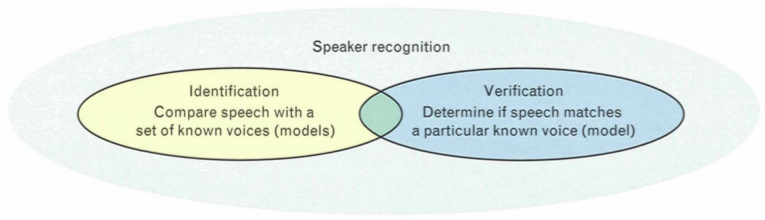
\includegraphics[width=0.75\textwidth]{speaker-recognition}
\end{figure}
\end{frame}

\begin{frame}
\frametitle{Dependência de texto}
\begin{description}
    \item[Dependente] Teste $\in$ Treinamento
    \pause
    \begin{itemize}
        \item Diversos graus de dependência
        \pause
        \item Teste $\not\in$ Treinamento $\implies$ Retreinamento
        \pause
    \end{itemize}
    \item[Independente] Teste $\neq$ Treinamento
    \pause
    \begin{itemize}
        \item Características não textuais
        \pause
        \item Presentes em diferentes sotaques e até \emph{gibberish}
    \end{itemize}
\end{description}
\end{frame}

\subsection{Modelos de Mistura Gaussiana}

\begin{frame}
\frametitle{Modelos de Mistura Gaussiana}
\begin{description}
    \item[GMM] Combinação de Gaussianas
    \pause
    \item[UBM] GMM gerado por diversas locuções de fundo
    \pause
    \item[AGMM] GMM adaptado a partir de um UBM
    \pause
    \item[FGMM] GMM utilizando Fractional Covariance Matrix (FCM)
\end{description}
\end{frame}

\subsection{Objetivos}

\begin{frame}
\frametitle{Objetivos}
\begin{description}
    \item Implementar sistemas de reconhecimento de locutor e analizar
    \pause
    \begin{itemize}
        \item Taxas de sucesso para \textbf{identificação}
        \pause
        \item Comparar identificação utilizando GMM e FGMM
        \pause
        \item Falsa detecção e falsa rejeição para \textbf{verificação}
        \pause
        \item Comparar verificação utilizando GMM e AGMM
    \end{itemize}
\end{description}
\end{frame}